\documentclass[../main.tex]{subfiles}

\begin{document}

\subsection{Gambler's Ruin}


\paragraph{} Supongamos que tienen \$100 y les ofrezco una apuesta donde vamos a tirar una moneda 100 veces seguidas. Cada vez que salga cara su riqueza sube un 50\%, y cada vez que salga cruz su riqueza decrementa un 40\%. ¿La tomarían?


\paragraph{} En un principio podemos calcular la ganancia esperada: Para la primera tirada tenemos un 50\% chances de ganar \$50, y un 50\% chances de perder \$40. Por lo que esperaríamos ganar:
\begin{gather*}
  \$50 \cdot 50\% + \$(-40) \cdot 50\% = \$5 = \$100 \cdot \%5
\end{gather*}

 El valor de la apuesta va a cambiar en las tiradas futuras, pero en todas vamos a tener una ganancia esperada del 5\%. Por lo que en promedio esperaríamos ganar un 5\% por tirada.

\paragraph{} Simulando esta apuesta para 10000 personas podemos ver que este promedio se cumple.
\begin{figure}[H]
  \centering
  \includegraphics[scale=0.7]{img/mean.pdf}
  \caption{Riqueza promedio entre 10000 personas jugando la apuesta.}
\end{figure}

\paragraph{} Pero mirándolo desde otra perspectiva, si revisamos la trayectoria de 20 personas elegidas al azar, notamos que aunque a un par les va bien la mayoría no alcanza tanta riqueza.

\begin{figure}[H]
  \centering
  \includegraphics[scale=0.7]{img/paths.pdf}
  \caption{Riqueza sobre el tiempo para 20 personas elegidas al azar.}
\end{figure}

De hecho, si lo miramos en escala logarítmica, se resalta que la mediana perdió casi todo su riqueza.

\begin{figure}[H]
  \centering
  \includegraphics[scale=0.7]{img/logPaths.pdf}
  \caption{Riqueza sobre el tiempo para 20 personas elegidas al azar comparadas con la promedio y la mediana.}
\end{figure}

\paragraph{} Una justificación de por qué sucede esto es revisar qué pasa después de dos tiradas.

Nuevamente arracamos con \$100, después de la primera tirada tenemos \%50 chance de tener \$150 y \%50 chance de tener \$60.

Ahora en esta segunda tirada:
\begin{itemize}
  \item Si teníamos \$150 tenemos \%50 chance de tener \$225 y \%50 chance de tener \$90.
  \item Y si teníamos \$60 tenemos \%50 chance de tener \$90 y \%50 chance de tener \$36.
\end{itemize}

Como se ve, después de dos tiradas hay tres casos posibles: O tenemos \$225 con probabilidad \(\frac{1}{4}\), o tenemos \$36 con probabilidad \(\frac{1}{4}\), o tenemos \$90 con probabilidad \(\frac{1}{2}\).

O sea que después de dos tiradas \(\frac{3}{4}\) de las veces perdimos dinero comparado con los \$100 iniciales.

Revisando más tiradas se ve que esto continúa, la mayoría de las veces perdemos (y rápido!).

\begin{figure}[H]
  \centering
  \begin{tikzpicture}
    \GVertex{\$100}{0}{4}{0}

    \GVertex{\$150}{-2}{2}{1}
    \GVertex{\$60}{2}{2}{2}

    \GVertex{\$225}{-2}{0}{3}
    \GVertex{\$90}{0}{0}{4}
    \GVertex{\$36}{2}{0}{5}

    \GEdge{$\frac{1}{2}$}{0}{1}
    \GEdge{$\frac{1}{2}$}{0}{2}

    \GEdge{$\frac{1}{2}$}{1}{3}
    \GEdge{$\frac{1}{2}$}{1}{4}

    \GEdge{$\frac{1}{2}$}{2}{4}
    \GEdge{$\frac{1}{2}$}{2}{5}
  \end{tikzpicture}
  \caption{Caminos posibles para dos tiradas}
\end{figure}

\paragraph{} A este problema se lo conoce como la \textbf{Gambler's Ruin} (Ruina del Apostador). Y es un ejemplo de un sistema no-ergódico.

Un sistema ergódico es un sistema donde el promedio individual sobre el tiempo converge al promedio grupal.  La mayoría de los sistemas reales son no-ergódicos.

Ver un problema así nos resalta que la probabilidad no es tan directa como la solemos pensar. No es suficiente con quedarse con el cálculo de la ganancia promedio.

\end{document}
